
\ifdefined\standalone 
\documentclass[12pt]{article}
\usepackage{graphicx}
\usepackage{float}
\usepackage[a4paper, margin=1in]{geometry}
\usepackage[utf8]{inputenc}
\usepackage{textcomp}
\usepackage{amsmath}
\usepackage{booktabs}
\usepackage{tikz}
\usepackage{enumitem}
\usetikzlibrary{decorations.pathmorphing,patterns}
\usepackage[hidelinks]{hyperref}
\usepackage[toc,page]{appendix}


\begin{document}
\fi


\section{Darcy Flow with Fixed Pressure}
\label{Darcy_pfixed}

This verification case examines the behaviour of the pressure solver in a porous material under steady one-dimensional gas flow with fixed pressure boundary conditions.  
A uniform porous layer of thickness $L = 10~\mathrm{cm}$ is considered (Figure~\ref{fig:configuration_darcy_pfixed}).  
The temperature is fixed at $T_0 = 300~\mathrm{K}$, and the permeability of the material is $\bar{K} = 5\cdot 10^{-10} \; \mathrm{m^{2}}$. The pressure is prescribed at both ends of the domain:
\[
P(0) = P_0 = 1~\mathrm{bar}, 
\qquad 
P(L) = P_L = 2~\mathrm{bar}.
\]

The gas kinematic viscosity is computed from the Chapman--Enskog model. In this verification case, the background gas and the diffusive species are identical.  
The kinematic viscosity is given by:
\begin{equation}
\nu = 0.018829 \, \frac{\sqrt{T_0^3 \frac{2}{M}}}{P\sigma^2 \, \Omega_D(\epsilon/k)} = \frac{\alpha}{P}
\end{equation}
where $M$ the molar mass of the gas, $\sigma$ and $\epsilon/k$ the Lennard--Jones parameters, and $\Omega_D$ the collision integral. The relevant thermophysical properties of the gas are summarized in Table~\ref{tab:properties_darcy_pfied}.


\begin{table}[H]
\centering
\caption{Gas properties}
\label{tab:properties_darcy_pfied}
\begin{tabular}{@{}llll@{}}
\toprule
$M$ ($\mathrm{g\cdot mol^{-1}}$) & $\sigma$($\mathrm{Å}$) & $\epsilon/k$ ($\mathrm{K}$) & $\alpha$ ($\mathrm{kg \cdot m \cdot s^{-1} }$)\\
\midrule
29 & 3.617 & 97 & 2.087 \\
\bottomrule
\end{tabular}
\end{table}


As demonstrated in ~\ref{ann:analytical_pressure2}, the analytical pressure profile is:

\begin{equation}
P(z)^2 = P_0^2 + \left(P_L^2 - P_0^2\right) \frac{z}{L}.
\end{equation}

And the corresponding mass flux is:
\begin{equation}
\dot{m}'' = \frac{\bar{K}}{2 \alpha L} \left(P_L^2 - P_0^2\right).
\end{equation}


Figures~\ref{fig:viscosity_darcy_pfixed}, \ref{fig:pressure_darcy_pfied}, and \ref{fig:flux_darcy_pfixed} present respectively the pressure distribution, the kinematic viscosity profile, and the mass flux comparison between the analytical solution and the Gpyro simulation.


\begin{figure}[H]
\centering

\begin{minipage}[t]{0.45\textwidth}
\centering
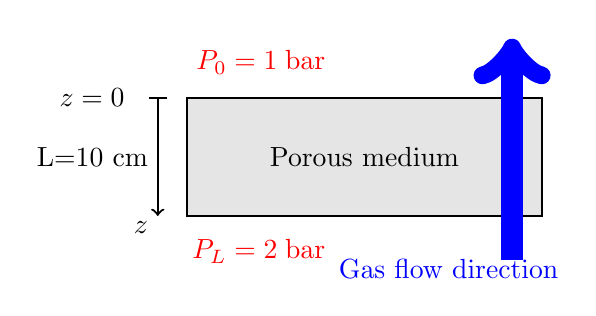
\begin{tikzpicture}[scale=0.75]


% Block
\draw[fill=gray!20,thick] (0,0) rectangle (6,2);
\node at (3,1) {Porous medium};

\draw[thick] (-0.35,2) -- (-0.65,2); 
\node[left] at (-0.9,2) {$z=0$};

\draw[thick,->] (-0.5,2) -- (-0.5,0);
\node[left] at (-0.5,1) {L=10~cm};
\node[left] at (-0.5,-0.2) {$z$};


% Top boundary
\node[red, left] at (2.5,2.6) {$P_0= 1 \;\mathrm{bar}$};
\node[red, left] at (2.5,-0.6) {$P_L= 2\; \mathrm{bar}$};

% Arrow showing flow direction
\draw[blue,line width=8pt,->] (5.5,-0.75) -- (5.5,3);
\node[blue,anchor=west] at (2.4,-0.9)
    {Gas flow direction};

\end{tikzpicture}



\caption{Configuration schematic}
\label{fig:configuration_darcy_pfixed}
\end{minipage}
\hfill
\begin{minipage}[t]{0.48\textwidth}
\centering
\includegraphics[width=\textwidth]{Pressure_darcy_fixed.png}
\caption{Pressure profile along the porous domain.}
\label{fig:pressure_darcy_pfied}
\end{minipage}

\end{figure}



\begin{figure}[H]
\centering
\begin{minipage}{0.48\textwidth}
\centering
\includegraphics[width=\textwidth]{Viscosity_darcy_fixed.png}
\caption{Kinematic viscosity profile.}
\label{fig:viscosity_darcy_pfixed}
\end{minipage}
\hfill
\begin{minipage}{0.48\textwidth}
\centering
\includegraphics[width=\textwidth]{flux_darcy_fixed.png}
\caption{Mass flux along the domain.}
\label{fig:flux_darcy_pfixed}
\end{minipage}
\end{figure}


\ifdefined\standalone
\end{document}
\fi



